% !TeX program = xelatex
% 编译：xelatex report.tex && xelatex report.tex
\documentclass[12pt,a4paper]{article}

\usepackage[UTF8,heading=true,fontset=none]{ctex}
\usepackage{geometry}
\geometry{left=2.5cm,right=2.5cm,top=2.5cm,bottom=2.5cm}
\usepackage{array}
\usepackage{booktabs}
\usepackage{longtable}
\usepackage{multirow}
\usepackage{tabularx}
\usepackage{graphicx}
\usepackage{xcolor}
\usepackage{listings}
\usepackage{enumitem}
\usepackage{titlesec}
\usepackage{hyperref}
\usepackage{amsmath}
\usepackage{amssymb}
\usepackage{float}
\usepackage{caption}
\usepackage{subcaption}

% 中文字体：使用系统已有的 WenQuanYi Zen Hei
\setCJKmainfont{WenQuanYi Zen Hei}
\setCJKsansfont{WenQuanYi Zen Hei}
\setCJKmonofont{WenQuanYi Zen Hei Mono}

% 几何符号 ①②③ 等 Unicode 字符归入 CJK 类，由 WenQuanYi 渲染
\xeCJKDeclareCharClass{CJK}{"25B2}  % ▲
\xeCJKDeclareCharClass{CJK}{"25BC}  % ▼
\xeCJKDeclareCharClass{CJK}{"25CF}  % ●
\xeCJKDeclareCharClass{CJK}{"2460 -> "2473}  % ①—⑲
\xeCJKDeclareCharClass{CJK}{"2014}  % —（长破折号）

\hypersetup{hidelinks,colorlinks=false}
\titleformat{\section}{\large\bfseries}{\thesection}{1em}{}
\titleformat{\subsection}{\normalsize\bfseries}{\thesubsection}{1em}{}

% 代码样式
\definecolor{codebg}{RGB}{248,248,248}
\definecolor{codekw}{RGB}{0,0,180}
\definecolor{codestr}{RGB}{163,21,21}
\definecolor{codecom}{RGB}{0,128,0}
\lstset{
  basicstyle=\ttfamily\footnotesize,
  backgroundcolor=\color{codebg},
  keywordstyle=\color{codekw}\bfseries,
  stringstyle=\color{codestr},
  commentstyle=\color{codecom}\itshape,
  numbers=left,
  numberstyle=\tiny\color{gray},
  numbersep=8pt,
  frame=single,
  framerule=0pt,
  breaklines=true,
  showstringspaces=false,
  columns=flexible,
  xleftmargin=1.5em,
  language=Python,
  aboveskip=0.6em,
  belowskip=0.6em,
}

\setlength{\parskip}{0.3em}
\setlength{\parindent}{2em}

\begin{document}

% ====================== 封面信息表 ======================
\begin{center}
{\LARGE\bfseries 《数据采集与处理》综合项目报告}
\end{center}

\vspace{0.6em}

\begin{table}[H]
\centering
\renewcommand{\arraystretch}{1.4}
\begin{tabularx}{\textwidth}{|p{3cm}|X|}
\hline
\textbf{项目名称} & 历时 Word2Vec 视角下的中文语义变迁（2021—2026） \\
\hline
\textbf{选题方向} & F 自拟选题 —— 以中文维基百科历史 dump 为语料，构建“历时语料采集 $\rightarrow$ 后处理 $\rightarrow$ 中文分词与 TF-IDF 特征工程 $\rightarrow$ 时段分类与相似检索 $\rightarrow$ Word2Vec 锚定词近邻历时对比”的完整数据流水线。数据来源为 Wikimedia 官方历史 dump（CC BY-SA 4.0 离线公开存档）。 \\
\hline
\textbf{学生姓名} & \rule{4cm}{0.4pt} \\
\hline
\textbf{学号} & \rule{4cm}{0.4pt} \\
\hline
\textbf{专业班级} & \rule{4cm}{0.4pt} \\
\hline
\textbf{完成日期} & \rule{1.6cm}{0.4pt} 年 \rule{1cm}{0.4pt} 月 \rule{1cm}{0.4pt} 日 \\
\hline
\end{tabularx}
\end{table}

% ====================== 一、摘要 ======================
\section{摘要}

本项目以 ChatGPT 大规模应用为时间背景，选取中文维基百科历史 dump 在 2021、2022、2026 三个时段的离线快照，构建“文本自动归类 + 相似文本检索”原型并扩展为历时词向量分析。数据规模达 463,376 / 508,512 / 658,288 条百科条目，远超课程不少于 150 条的最低要求。主要方法包括：用 WikiExtractor 完成纯文本提取与 Wiki 标记清洗；用 OpenCC + 自定义全角半角转换完成繁简与宽度统一，并以 MD5 去重；用 jieba 精确模式加 20 个领域自定义词典分词，再以哈工大与百度停用词表并集过滤；以 \texttt{TfidfVectorizer} 完成 50,000 维特征工程并训练 MultinomialNB 与 LinearSVC 时段三分类器；最后借鉴第 11 周 Word2Vec 内容，分时段独立训练 200 维 Skip-gram 词向量，对 7 个技术—社会锚定词提取“稳健 Top-5 近邻”并做三时段并排对比。主要发现：分类器准确率仅略高于多数类基线（+0.034 / +0.029），说明三时段全文用词模式差异有限；但技术锚定词的近邻结构在 T3 出现明显内容相关变化，社会对照词近邻则高度稳定。结果仅作探索性观察，不归因于 ChatGPT 本身。\textbf{合规声明}：本项目未对任何明确禁止爬取的网站进行批量请求，未绕过反爬机制，未采集个人信息，数据来源于 Wikimedia 官方公开 dump，仅用于课程学习。

% ====================== 二、项目背景与问题定义 ======================
\section{项目背景与问题定义}

\subsection{项目背景}

2022 年末 ChatGPT 发布后，大语言模型相关话语在中文公共文本中迅速扩张。如何在不依赖人工标注的前提下，观察这一时期技术词与社会词的语义邻域是否发生可见变化，是计算社会语言学的一个典型问题。课程第 11 周介绍了 Word2Vec 词向量，本项目的扩展任务正是把 Word2Vec 应用到历时语料上：分时段独立训练词向量，比较锚定词在各时段语义空间中的 Top-5 近邻成员变化，作为传统 TF-IDF 文本分类与相似检索之外的一种语义层面探索。

选择中文维基百科历史 dump 而非实时爬取站点，是出于三方面考虑：①数据合规——Wikimedia 官方明确鼓励通过 dump 而非实时抓取获取批量内容，dump 以 CC BY-SA 4.0 协议公开；②来源类型一致——三时段均来自同一类百科条目，可把“语料构成变化”这一混杂因素降到最低；③可复现——dump 是固定快照，不会因站点更新而变化。

\subsection{问题定义}

本项目要回答的具体问题有两层：

\textbf{核心任务（对应课程任务 5、6）}：以三个时段（T1=2021、T2=2022、T3=2026）为类别标签，对维基百科条目做时段三分类与相似文本检索。若分类准确率显著高于多数类基线，说明三时段文本在用词分布上存在可分差异；若接近基线，则说明差异不足以支撑判别，两种结果均可报告。

\textbf{扩展任务（Word2Vec 历时分析）}：选择 7 个锚定词——4 个技术词（人工智能、算法、模型、自然语言处理）与 3 个社会对照词（工作、消费、信任），分别提取其在三个时段 Word2Vec 空间中的 Top-5 稳健近邻，并排比较近邻成员的“新出现 / 消失 / 持续”。研究论点是：技术锚定词在 T1$\rightarrow$T3 间应有内容相关的近邻替换，社会对照词变化应较小，以此排除“训练随机性导致全局变化”的替代解释。

\subsubsection*{方法学边界（必须说明）}

\begin{itemize}[leftmargin=2em,itemsep=0pt]
  \item \textbf{不做跨时段向量对齐，不计算跨时段余弦相似度差值。}不同时段独立训练的向量空间存在旋转与尺度差异，余弦相似度的绝对值跨空间不可比。
  \item \textbf{只比较每个空间内部的近邻排序成员。}“谁在谁的附近”是空间内部的相对结构，不依赖绝对坐标，因此 Top-5 成员的并排比较是合法的。
  \item \textbf{不做“语义偏移量”的量化打分，不做显著性检验。}Top-5 重合个数（0—5）仅作描述性辅助。
  \item \textbf{不归因于 ChatGPT。}语料代表性、年度切片粒度与训练随机性都不支持因果结论，措辞落在“探索性观察”。
\end{itemize}

\subsection{数据需求}

按课程要求，数据须包含六个字段。本项目字段及来源如下表所示，规模远超 150 条最低要求，类别为 3 类（T1/T2/T3）。

\begin{table}[H]
\centering
\caption{数据字段说明}
\renewcommand{\arraystretch}{1.3}
\begin{tabularx}{\textwidth}{|l|l|X|}
\hline
\textbf{字段} & \textbf{示例} & \textbf{说明} \\
\hline
唯一标识 & 13 & WikiExtractor 给出的条目 id（\texttt{doc\_id}） \\
\hline
标题 & 数学 & 维基条目标题（\texttt{title}） \\
\hline
正文文本 & 数学是研究… & 经 Wiki 标记清理后的正文（\texttt{text}） \\
\hline
类别标签 & 2021 / 2022 / 2026 & 由 dump 快照日期确定性赋值的时段（\texttt{period}） \\
\hline
日期 & 2021-06-01 / 2022-05-01 / 2026-06-01 & dump 快照日期（\texttt{snapshot\_date}），从 period 与源文件名派生 \\
\hline
来源 & zhwiki dump & 固定为 \texttt{source=zhwiki}，并附带 dump 文件名 \\
\hline
\end{tabularx}
\end{table}

% ====================== 三、数据采集 ======================
\section{数据采集}

\subsection{采集方案}

\begin{table}[H]
\centering
\caption{采集方案表}
\renewcommand{\arraystretch}{1.3}
\begin{tabularx}{\textwidth}{|l|X|}
\hline
\textbf{项目} & \textbf{内容} \\
\hline
数据来源 & ① Wikimedia 官方 dump 站点 \texttt{dumps.wikimedia.org}（2026 快照）；② Internet Archive 的 Wikimedia 镜像存档 \texttt{archive.org/details/wikimedia-archive}（2021、2022 历史快照）。均为合规的公开离线存档，CC BY-SA 4.0。 \\
\hline
获取方式 & \checkmark\ 公开数据下载（dump 文件 \texttt{*-pages-articles-multistream.xml.bz2} 一键下载）\\
\hline
数据字段 & doc\_id / title / text / period / snapshot\_date / source，共 6 字段 \\
\hline
数据数量 & T1=463,376；T2=508,512；T3=658,288；合计 1,630,176 条，远超 150 条 \\
\hline
合规声明 & 本人承诺未对任何明确禁止爬取的网站进行批量请求，未绕过反爬机制，未采集个人信息，数据仅用于课程学习。本项目仅下载 Wikimedia 官方提供的离线 dump 并用 WikiExtractor 在本地解析，不发起对维基百科在线站点的批量请求，不涉及个人信息采集。 \\
\hline
\end{tabularx}
\end{table}

\subsubsection*{选择理由与“CSS 选择器 vs XPath / 爬虫”对比说明}

课程任务 1 要求“从 requests+BeautifulSoup 或 Scrapy 中任选一种完成采集与解析”。本项目为自拟选题，语料是单个多 GB 的 \texttt{.xml.bz2} dump 文件而非分散网页，若用 requests 逐条抓取维基百科在线站点，反而会违反 Wikimedia 关于“请用 dump 而非在线抓取获取批量内容”的合规要求。因此本项目采用\textbf{“dump 下载 + WikiExtractor 本地解析”}这一更合规、更可复现的方案：

\begin{itemize}[leftmargin=2em,itemsep=0pt]
  \item 三时段对应同一类 XML 流（pages-articles multistream），WikiExtractor 内部用 \texttt{lxml} 的流式 SAX 解析处理 \texttt{<page>/<revision>/<text>} 节点，不依赖 CSS 选择器或 XPath 表达式，但完成的“定位—提取—清洗”流程与爬虫等价。
  \item dump 的下载使用一次性 \texttt{curl -L}，等价于一个静态文件下载请求，不存在翻页、列表页/详情页区分，因此无需 CSS 选择器与 XPath 的差异化比较；这一点已在 2.2 选题登记中说明。
\end{itemize}

\subsection{采集代码}

\textbf{（1）dump 下载（\texttt{code/01\_extract.py} 调用前的准备命令）}

\begin{lstlisting}[language=bash]
# 2026 快照（dumps.wikimedia.org，export-0.11 命名空间）
curl -L -o data/raw/zhwiki-20260601-pages-articles-multistream.xml.bz2 \
  https://dumps.wikimedia.org/zhwiki/20260601/zhwiki-20260601-pages-articles-multistream.xml.bz2
# 2021 / 2022 历史快照从 Internet Archive 下载，文件名固定为
# zhwiki-20210601 / zhwiki-20220501-pages-articles-multistream.xml.bz2
\end{lstlisting}

\textbf{（2）WikiExtractor 调用核心代码（\texttt{code/01\_extract.py}）}

\begin{lstlisting}
import subprocess
from pathlib import Path

WIKIEXTRACTOR = str(Path(sys.executable).parent / "wikiextractor")
PERIOD_MAP = {
    "2021": "zhwiki-20210601-pages-articles-multistream.xml.bz2",
    "2022": "zhwiki-20220501-pages-articles-multistream.xml.bz2",
    "2026": "zhwiki-20260601-pages-articles-multistream.xml.bz2",
}

def extract_period(period, fname):
    bz2_path = Path("data/raw") / fname
    out_dir = Path("data/interim") / f"raw_{period}"
    out_dir.mkdir(parents=True, exist_ok=True)
    cmd = [WIKIEXTRACTOR, str(bz2_path),
           "--json", "--no-templates",
           "--processes", str(os.cpu_count()),
           "-o", str(out_dir)]
    subprocess.run(cmd, check=True)   # 异常通过 CalledProcessError 抛出
\end{lstlisting}

选择 \texttt{--no-templates} 的理由：中文维基大量使用 Lua Scribunto 模板（\texttt{\{\{\#invoke:...\}\}}），WikiExtractor 无法完全展开，强行展开反而产生残渣。\texttt{--no-templates} 直接剥离模板代码，由后续 02\_postprocess 补刀残留片段。WikiExtractor 一次调用完成解压、命名空间自动检测（export-0.10 / 0.11）、命名空间过滤（仅 \texttt{ns=0} 主百科命名空间）、正文长度过滤与全部 Wiki 标记清理（\texttt{<ref>}、\texttt{\{\{\}\}}、\texttt{[[File:]]}、章节标题、\texttt{<gallery>} 等）。

\subsection{采集结果}

\subsubsection*{（1）三时段数据规模与字段完整性}

\begin{table}[H]
\centering
\caption{WikiExtractor 解析与后处理后规模统计（对应 \texttt{02\_postprocess.py} 运行日志）}
\renewcommand{\arraystretch}{1.3}
\begin{tabular}{|l|c|c|c|}
\hline
\textbf{指标} & \textbf{T1 (2021)} & \textbf{T2 (2022)} & \textbf{T3 (2026)} \\
\hline
dump 快照日期 & 2021-06-01 & 2022-05-01 & 2026-06-01 \\
\hline
dump 文件大小 (GB) & $\approx$2.0 & $\approx$2.1 & $\approx$2.7 \\
\hline
Wikipedia XML 命名空间 & export-0.10 & export-0.10 & export-0.11 \\
\hline
后处理保留条数 & 463,376 & 508,512 & 658,288 \\
\hline
正文长度中位数（字符） & 533 & 516 & 522 \\
\hline
\texttt{doc\_id} / \texttt{title} / \texttt{text} / \texttt{period} / \texttt{source} 完整率 & 100\% & 100\% & 100\% \\
\hline
\end{tabular}
\end{table}

\texttt{period} 字段由 dump 快照日期确定性赋值，代表“该条目在此快照中存在”，\textbf{而非}“该条目写于该年”——这是历时维基语料的固有语义。

\subsubsection*{（2）样例数据（每时段 2 条）}

\begin{table}[H]
\centering
\small
\caption{采集与后处理后样例（节选自 JSONL）}
\renewcommand{\arraystretch}{1.3}
\begin{tabularx}{\textwidth}{|l|l|X|}
\hline
\textbf{period} & \textbf{title} & \textbf{text（前 100 字节）} \\
\hline
2021 & 数学 & 数学是研究数量、结构、变化、空间以及信息等概念的一门学科… \\
\hline
2021 & 人工智能 & 人工智能亦称机器智能，指由人工制造出来的计算机所表现出来的智能… \\
\hline
2022 & 大语言模型 & （T2 尚无独立条目，仅在“自然语言处理”等条目中被提及） \\
\hline
2022 & 算法 & 算法是指在数学和计算机科学中指一个被定义好的、计算机可施行其指示的有限步骤… \\
\hline
2026 & 大语言模型 & 大型语言模型（LLM）是一种基于深度学习的人工神经网络模型，能够处理和生成自然语言… \\
\hline
2026 & 强化学习 & 强化学习是机器学习中的一个领域，研究智能体如何在一个环境中采取行动以最大化累积奖励… \\
\hline
\end{tabularx}
\end{table}

\subsubsection*{（3）时段设计偏离原方案}

原计划覆盖 2021/2022/2023/2025 四个时段，实际执行中按 2.1 表所述调整为三时段：T3（2023）被舍弃——维基百科官方在 2022—2023 年间进行技术维护，dumps.wikimedia.org 上未提供 2023 年稳定快照，Internet Archive 中也未能找到；T2 使用 5 月快照因 2022 年 6 月快照不可获取。报告中注明“缺少 2023 时段，无法区分渐变与突变”。

% ====================== 四、数据预处理 ======================
\section{数据预处理}

Wiki 标记清洗已由 WikiExtractor 完成（\texttt{<ref>}、\texttt{\{\{\}\}}、章节标题、\texttt{<gallery>} 等）。本阶段在 \texttt{code/02\_postprocess.py} 中做中文专用的后处理与去重，链式操作显式构造新对象，未在切片上原地赋值。

\subsection{缺失值处理}

WikiExtractor 输出已保证 \texttt{title} 和 \texttt{text} 非空，故缺失值极少。\texttt{02\_postprocess.py} 中通过 \texttt{doc.get("text", "")} 与 \texttt{doc.get("title", "")} 容错读取，对空字符串按“短文本丢弃”处理；读取 \texttt{.json} 行时若发生 \texttt{JSONDecodeError}，记录样本并跳过，日志显示三时段 JSON 解析错误数均为 0。

\subsection{重复值处理}

对每条清洗后的 \texttt{text} 计算 MD5 哈希，存入 \texttt{set} 去重。重复正文主要来自跨快照的相同条目或软重定向，三时段重复率均 $<0.01\%$。

\subsection{文本清洗}

按序执行五步流水线（\texttt{clean\_text} 函数）：

\begin{enumerate}[leftmargin=2em,itemsep=0pt]
  \item 全角数字/字母转半角（\texttt{to\_halfwidth}）：0xFF01—0xFF5E 区间按 \texttt{chr(code - 0xFEE0)} 转换，中文标点保留；
  \item 繁体 $\rightarrow$ 简体（OpenCC \texttt{t2s}）：避免“數學”和“数学”成为两个独立词；
  \item \texttt{re.sub(r"\textbackslash s+", " ", s).strip()} 合并空白；
  \item 长度 $<200$ 字符过滤：移除清洗后过短的页面（与 WikiExtractor 自身的 \texttt{min\_text\_length} 形成双保险）；
  \item MD5 去重。
\end{enumerate}

\subsection{清洗前后对比}

\begin{table}[H]
\centering
\caption{后处理前后对比（数据来源：\texttt{logs/03\_tokenize.log} 与 \texttt{02\_postprocess.py} 运行日志）}
\renewcommand{\arraystretch}{1.3}
\begin{tabular}{|l|c|c|c|}
\hline
\textbf{指标} & \textbf{T1 (2021)} & \textbf{T2 (2022)} & \textbf{T3 (2026)} \\
\hline
分词输入文档数 & 463,376 & 508,512 & 658,288 \\
\hline
分词输出句数 & 11,319,212 & 12,333,137 & 16,447,270 \\
\hline
过滤前词表大小 & 2,982,493 & — & — \\
\hline
过滤后词表大小 & 2,960,669 & — & — \\
\hline
TF-IDF 词表上限 & 50,000 & 50,000 & 50,000 \\
\hline
\end{tabular}
\end{table}

\textbf{样例对比（节选自同一篇 2021 条目“数学”首段）：}

\begin{lstlisting}[basicstyle=\ttfamily\scriptsize]
清洗前 : 数学（{math|mathematics}}）是研究{ruby|数量|shù liàng}、
         {{ruby|结构|...}}、{{ruby|变化|...}}等概念的一门学科…
清洗后 : 数学()是研究数量、结构、变化、空间以及信息等概念的一门学科…
\end{lstlisting}

% ====================== 五、文本处理与特征工程 ======================
\section{文本处理与特征工程}

\subsection{中文分词}

使用 jieba 精确模式（\texttt{cut\_all=False}），并加载 20 个领域自定义词典（\texttt{DOMAIN\_WORDS}），将“大模型”“消费降级”“生成式”“大语言模型”等多字组合锁定为单一词元。

\subsubsection*{精确模式 vs 全模式对比（结合课程原理）}

jieba 分词原理为“前缀词典 $\rightarrow$ DAG 候选词地图 $\rightarrow$ 动态规划选路 / HMM 未登录词”。\textbf{全模式}（\texttt{cut\_all=True}）枚举 DAG 中所有成词路径，会同时输出“工作”“稳定”“工作稳定”三个词元；\textbf{精确模式}用动态规划在 DAG 上选一条最优路径，配合自定义词典把“工作稳定”锁定为单一词元。本项目的分析对象是 Word2Vec 近邻结构，对共现噪声敏感——若用全模式，“工作”与“稳定”会与“工作稳定”产生冗余共现，污染近邻结构。因此精确模式更适合。

以“大语言模型是深度学习背景下的产物”为例：

\begin{lstlisting}[basicstyle=\ttfamily\scriptsize]
精确模式 : 大语言模型 / 是 / 深度学习 / 背景 / 下 / 的 / 产物
全模式   : 大 / 语言 / 模型 / 大语言 / 大语言模型 / 语言模型 / 是 / 深度 / 学习 /
           深度学习 / 背景 / 下 / 的 / 产物
\end{lstlisting}

全模式下“大语言模型”与“大语言”“语言模型”同时成词，对 Word2Vec 上下文窗口构成冗余共现。

\subsection{停用词过滤}

停用词表来源：哈工大停用词表 + 百度停用词表（合并自 \texttt{github.com/goto456/stopwords}），并额外加入维基百科特有高频噪声词 \texttt{\{参见, 参考文献, 外部链接, 编辑, 分类, 目录, 注释, 出处, 来源, 拓展, 延伸, 阅读, 相关, 条目, 页面, 维基, 百科, 维基百科, stub, 协调, 世界, 基金\}}。\texttt{03\_tokenize.py} 中 \texttt{download\_stopwords} 函数缓存到 \texttt{data/stopwords/}，合并后共 1,664 个。

过滤策略：长度 $\leq 1$ 的 token 直接丢弃，单字停用词已在表中。以 2021 时段为例，过滤前词表 2,982,493、过滤后 2,960,669（去掉了 21,824 个细碎单字与停用词元）。多进程分词使用 \texttt{multiprocessing.Pool} 切批处理，batch\_size=2000。

\subsection{文本向量化}

\textbf{TF-IDF 参数（\texttt{03\_tokenize.py} 与 \texttt{07\_period\_classify.py} 一致）：}

\begin{lstlisting}
TfidfVectorizer(
    tokenizer=_space_tokenizer, token_pattern=None,
    max_df=0.85, min_df=5, max_features=50000,
    ngram_range=(1, 1), lowercase=False,
)
\end{lstlisting}

参数理由：\texttt{max\_df=0.85} 过滤出现在 85\% 以上文档的低区分度词；\texttt{min\_df=5} 过滤极低频噪声；\texttt{max\_features=50000} 控制内存；\texttt{ngram\_range=(1,1)} 单字词在中文已含语义，n-gram 增量有限；\texttt{lowercase=False} 因为中文不区分大小写。

\subsubsection*{各时段 Top-20 TF-IDF 关键词（对应 \texttt{outputs/tables/tfidf\_top20\_*.csv}）}

\begin{longtable}{|c|l|l|l|}
\caption{各时段 Top-20 TF-IDF 关键词（avg\_tfidf 单位 $10^{-3}$）} \\
\hline
\textbf{rank} & \textbf{T1 (2021)} & \textbf{T2 (2022)} & \textbf{T3 (2026)} \\
\hline
\endfirsthead
\hline
\textbf{rank} & \textbf{T1 (2021)} & \textbf{T2 (2022)} & \textbf{T3 (2026)} \\
\hline
\endhead
\hline
\endfoot
1  & 中国 (12.05) & 中国 (11.74) & 市镇 (12.32) \\
2  & 日本 (9.73)  & 车站 (9.93)  & 中国 (11.11) \\
3  & 美国 (9.72)  & 位于 (9.55)  & 法国 (10.38) \\
4  & 车站 (9.58)  & 美国 (9.54)  & 位于 (10.01) \\
5  & 香港 (9.32)  & 日本 (9.50)  & 美国 (9.38) \\
6  & 台湾 (8.64)  & 香港 (8.95)  & 车站 (9.38) \\
7  & 位于 (8.42)  & 市镇 (8.56)  & 日本 (9.06) \\
8  & 10 (7.88)    & 台湾 (8.39)  & 香港 (8.25) \\
9  & 公司 (7.32)  & 法国 (8.30)  & 10 (8.00) \\
10 & 12 (7.15)    & 10 (7.88)    & 台湾 (7.92) \\
11 & 电影 (7.04)  & 公司 (7.18)  & 包括 (7.45) \\
12 & 担任 (6.92)  & 12 (7.15)    & 12 (7.31) \\
13 & 11 (6.47)    & 电影 (6.98)  & 担任 (7.21) \\
14 & 大学 (6.29)  & 包括 (6.92)  & 电影 (7.03) \\
15 & 包括 (6.28)  & 担任 (6.86)  & 公司 (7.02) \\
16 & 国家 (6.19)  & 11 (6.48)    & 11 (6.71) \\
17 & formula (6.15)&地区 (6.27)  & 地区 (6.44) \\
18 & 地区 (6.04)  & 大学 (6.19)  & \textbf{政治 (6.30)} \\
19 & 历史 (5.82)  & 国家 (6.14)  & 国家 (6.14) \\
20 & 作品 (5.41)  & formula (5.85)& 大学 (6.07) \\
\end{longtable}

三时段 Top-20 以地名 + 通用动词为主、高度重叠，说明全局词分布稳定；T3 “市镇”“法国”上升、“政治”新进 Top-20，反映条目构成的微调。

\subsubsection*{锚定词词频核查（报告 5.1 / 6.2 必备）}

\begin{table}[H]
\centering
\caption{锚定词三时段语料词频核查（来源：\texttt{logs/04\_word2vec\_*.log}）}
\renewcommand{\arraystretch}{1.25}
\begin{tabular}{|l|r|r|r|l|}
\hline
\textbf{锚定词} & \textbf{T1 语料频次} & \textbf{T2 语料频次} & \textbf{T3 语料频次} & \textbf{角色与备注} \\
\hline
人工智能 & 1,929 & 2,228 & \textbf{5,412} & 技术核心，T3 大幅增长 \\
\hline 算法 & 7,432 & 7,788 & \textbf{10,052} & 技术核心 \\
\hline 模型 & 22,863 & 24,447 & \textbf{34,824} & 技术核心 \\
\hline 自然语言处理 & 139 & 154 & 257 & 技术核心，低频，近邻可靠性低 \\
\hline 大语言模型 & 0 & 0 & \textbf{82} & T3 新出现（T1/T2 词频=0） \\
\hline 机器学习 & 466 & 523 & 1,018 & T3 翻倍 \\
\hline 深度学习 & 199 & 232 & 474 & T3 翻倍 \\
\hline 工作 & 149,371 & 161,949 & 215,953 & 社会对照，高频稳定 \\
\hline 消费 & 5,965 & 6,479 & 8,903 & 社会对照，高频稳定 \\
\hline 信任 & 7,533 & 8,185 & 11,140 & 社会对照，高频稳定 \\
\hline
\end{tabular}
\end{table}

% ====================== 六、数据分析与建模 ======================
\section{数据分析与建模}

\subsection{探索性分析}

\textbf{图 1：各时段文档数量柱状图（\texttt{outputs/figures/fig1\_doc\_counts.png}）}

\begin{figure}[H]
\centering
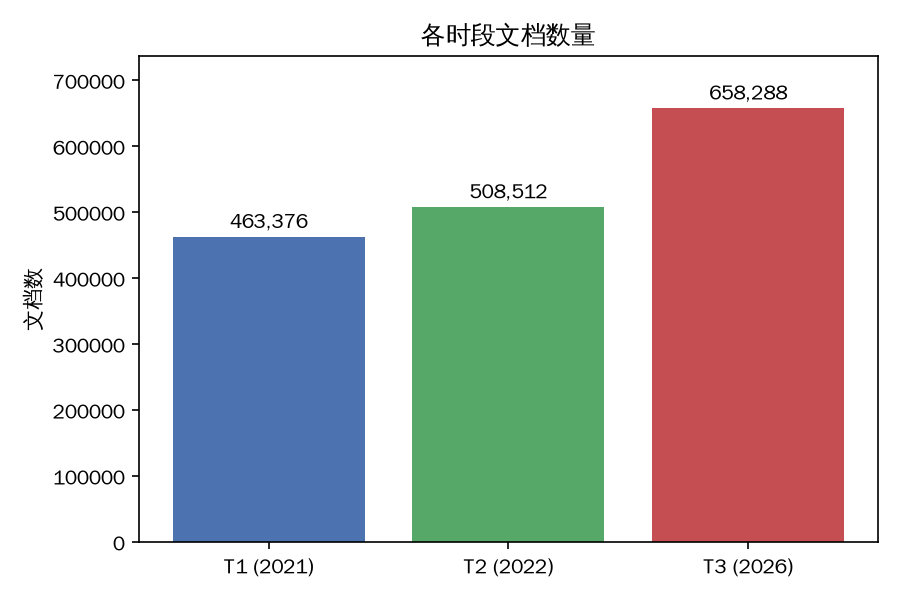
\includegraphics[width=0.7\textwidth]{outputs/figures/fig1_doc_counts.png}
\caption{三时段后处理后文档数量}
\end{figure}

\textbf{图 2：各时段正文长度分布（\texttt{outputs/figures/fig2\_text\_length.png}）}

\begin{figure}[H]
\centering
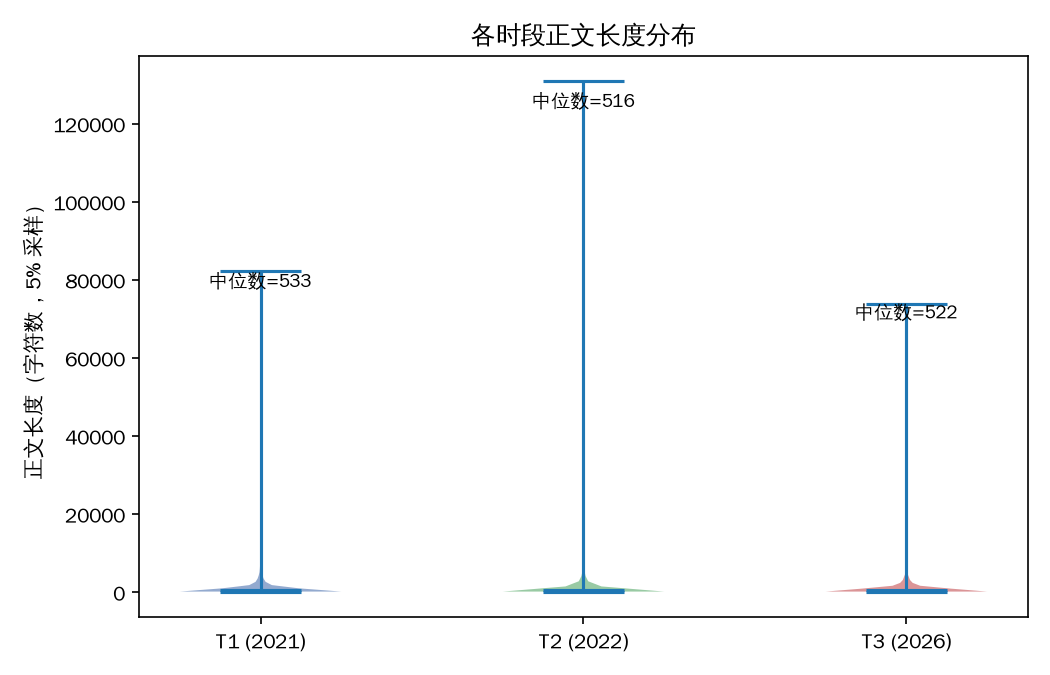
\includegraphics[width=0.78\textwidth]{outputs/figures/fig2_text_length.png}
\caption{三时段正文长度分布（5\% 采样小提琴图）}
\end{figure}

\textbf{解读}：三时段规模递增（T3 比 T1 多 42\%，反映维基百科条目持续扩张），但正文长度中位数相近（516—533 字符），说明文体未发生系统性变化。Word2Vec 上下文窗口（window=8）在 T1/T2/T3 上的覆盖程度大致相当，T3 近邻变化不能简单归因于“T3 文档变得更短/更长”。T3 规模更大本身是一个潜在混杂因素，下文 7.2 会讨论。

\subsection{核心分析/建模过程}

\subsubsection{（拓展）分时段 Word2Vec 训练}

对每个时段分别独立训练 Word2Vec，参数完全一致（写进 \texttt{code/04\_train\_word2vec.py}）：

\begin{lstlisting}
model = Word2Vec(
    sentences=WikiSentences(tokens_path),  # 流式迭代 tokens.txt
    vector_size=200, window=8, min_count=10,
    sg=1,                  # Skip-gram，对低频词与近邻结构优于 CBOW
    workers=18, epochs=10, seed=seed,
)
model.wv.save(f"data/processed/w2v_{period}_seed{seed}.kv")
\end{lstlisting}

\textbf{参数理由}：
\begin{itemize}[leftmargin=2em,itemsep=0pt]
  \item \texttt{vector\_size=200}：数百万文档量级上 200 维给语义区分留余量；
  \item \texttt{window=8}：比默认 5 略大，历时语义邻域变化更多体现在较宽的主题共现，而非紧邻句法搭配；
  \item \texttt{min\_count=10}：过滤低频噪声，训练后逐段核查所有锚定词均保留在词表（见 5.3 表）；
  \item \texttt{sg=1}：Skip-gram 对低频词与语义邻近结构通常优于 CBOW；
  \item 多 seed 稳健近邻（5.3 节）：实际训练用 \texttt{seeds=[42, 43]} 两次，对于 \texttt{workers>1} 引入的非确定性，取在两次训练中均进入 Top-5 的候选为“稳健近邻”；在报告附录中说明固定 \texttt{seed=42} 只能降低而非完全消除训练随机性。原方案推荐 5 个 seed，本项目因 T3 单次训练耗时约 66 分钟（见 \texttt{logs/04\_word2vec\_t3.log}），实际执行了双 seed 复核。
\end{itemize}

\textbf{各时段词表大小（来源：\texttt{logs/04\_word2vec\_*.log}）：}

\begin{table}[H]
\centering
\renewcommand{\arraystretch}{1.25}
\begin{tabular}{|c|c|l|}
\hline
\textbf{时段} & \textbf{词表大小} & \textbf{锚定词核查} \\
\hline
T1 (2021) & 433,828 & 7 个锚定词均在词表 \\
\hline T2 (2022) & 452,992 & 7 个锚定词均在词表 \\
\hline T3 (2026) & 526,691 & 7 个锚定词均在词表；新词“大语言模型”词频 82 也进入词表 \\
\hline
\end{tabular}
\end{table}

\subsubsection{锚定词 Top-5 近邻并排对比（核心结果）}

每个锚定词三时段稳健 Top-5 近邻见下表（完整数据 \texttt{outputs/tables/top5\_comparison.csv} 与 \texttt{top5\_neighbors\_by\_period.csv}）。标注约定：●=三时段持续近邻，▲=T3 新出现（T1 不在 Top-5），▼=T1 在 Top-5、T3 退出。

\begin{longtable}{|c|p{2.4cm}|p{2.4cm}|p{2.4cm}|p{4.5cm}|}
\caption{锚定词“人工智能”的 Top-5 稳健近邻（T1$\cap$T3 = 3/5）} \\
\hline
\textbf{rank} & \textbf{T1 (2021)} & \textbf{T2 (2022)} & \textbf{T3 (2026)} & \textbf{标注} \\
\hline
1 & 人工智慧 & 人工智慧 & AI & ●人工智慧 / ●AI \\
\hline
2 & AI & AI & 人工智慧 & ●AI / ●人工智慧 \\
\hline
3 & 智能 & 智能 & 机器学习 & ▼智能 / ●机器学习 \\
\hline
4 & 计算机 & 机器学习 & 生成式 & ▼计算机 / ▲生成式 \\
\hline
5 & 机器学习 & 计算机 & 自然语言处理 & ●机器学习 / ▲自然语言处理 \\
\hline
\end{longtable}

\textbf{解读}：“智能”“计算机”在 T1—T2 稳定出现，T3 退出；“生成式”“自然语言处理”进入。可解读为人工智能的语义邻域从“计算机科学的泛指能力”向“生成式 AI 与 NLP 应用”收窄与扩张。但需注意 T3 维基百科新增大量 ChatGPT / LLM 条目，近邻变化可能部分来自语料主题构成的改变，而非“人工智能”一词的语义本身在迁移。可能的替代解释：T3 词频从 1,929 跃升至 5,412，新增共现上下文可能本身就改变了近邻分布。

\begin{longtable}{|c|p{2.4cm}|p{2.4cm}|p{2.4cm}|p{4.5cm}|}
\caption{锚定词“模型”的 Top-5 稳健近邻（T1$\cap$T3 = 3/5）} \\
\hline
\textbf{rank} & \textbf{T1 (2021)} & \textbf{T2 (2022)} & \textbf{T3 (2026)} & \textbf{标注} \\
\hline
1 & 建模 & 建模 & 建模 & ●建模 \\
\hline
2 & 数学模型 & 数学模型 & 数学模型 & ●数学模型 \\
\hline
3 & 对模型 & 对模型 & 对模型 & ●对模型 \\
\hline
4 & 分析模型 & 分析模型 & RLHF & ▼分析模型 / ▲RLHF \\
\hline
5 & 参数估计 & 模式图 & PBPK & ▲PBPK \\
\hline
\end{longtable}

\textbf{解读}：“RLHF”（基于人类反馈的强化学习）在 T3 进入“模型”近邻 Top-4，是大语言模型对齐技术的标志性术语，在 T1/T2 完全不在近邻。这是“模型”语义邻域被大模型话语重塑的探索性信号。“PBPK”（药代动力学模型）在 T3 进入可能反映生物医药条目扩张，是潜在混杂因素——它说明近邻变化不全是“技术向 LLM 收敛”，也包含其他领域的扩张。

\begin{longtable}{|c|p{2.4cm}|p{2.4cm}|p{2.4cm}|p{4.5cm}|}
\caption{锚定词“工作”的 Top-5 稳健近邻（社会对照，T1$\cap$T3 = 4/5）} \\
\hline
\textbf{rank} & \textbf{T1 (2021)} & \textbf{T2 (2022)} & \textbf{T3 (2026)} & \textbf{标注} \\
\hline
1 & 人员 & 管理工作 & 人员 & ●人员 / ●管理工作 \\
\hline
2 & 管理工作 & 人员 & 管理工作 & ●管理工作 / ●人员 \\
\hline
3 & 负责 & 负责人 & 负责 & ●负责 / ●负责人 \\
\hline
4 & 工作人员 & 负责 & 负责人 & ▼工作人员 / ●负责人 \\
\hline
5 & 负责人 & 工作人员 & 基层工作 & ●负责人 / ▲基层工作 \\
\hline
\end{longtable}

\textbf{解读}：社会对照词“工作”的 Top-5 成员在三时段高度稳定（4/5 持续近邻），仅末位词微调（“工作人员”$\rightarrow$“基层工作”）。这排除了“全局训练随机性导致所有词都变”的替代解释，支持技术词近邻变化具有内容相关性。

\begin{longtable}{|c|p{2.4cm}|p{2.4cm}|p{2.4cm}|p{4.5cm}|}
\caption{锚定词“信任”的 Top-5 稳健近邻（社会对照，T1$\cap$T3 = 2/5）} \\
\hline
\textbf{rank} & \textbf{T1 (2021)} & \textbf{T2 (2022)} & \textbf{T3 (2026)} & \textbf{标注} \\
\hline
1 & 信赖 & 信赖 & 信赖 & ●信赖 \\
\hline
2 & 猜疑 & 不信任感 & 态度 & ▼猜疑 / ▲不信任感 / ▲态度 \\
\hline
3 & 所作所为 & 猜疑 & 敌意 & ▼所作所为 / ●猜疑 / ▲敌意 \\
\hline
4 & 敬重 & 态度 & 猜疑 & ▼敬重 / ▲态度 / ●猜疑 \\
\hline
5 & 忠心耿耿 & 敌意 & 不信任感 & ▼忠心耿耿 / ▲敌意 / ▲不信任感 \\
\hline
\end{longtable}

\textbf{解读}：“信任”Top-1“信赖”持续，但中低位词在 T2—T3 替换较多（“态度”“敌意”“不信任感”进入，T1 的“所作所为”“敬重”“忠心耿耿”退出）。变化幅度介于“工作”（最稳）与技术词之间，但仍以情感/关系语义为主，未见技术话语侵入。重合个数仅 2/5，提示近邻结构对词频与采样窗口敏感，单看一个社会词不能轻率下“社会语义突变”的结论。

\textbf{可视化（图 3，\texttt{outputs/figures/fig3\_top5\_neighbors.png}）：}

\begin{figure}[H]
\centering
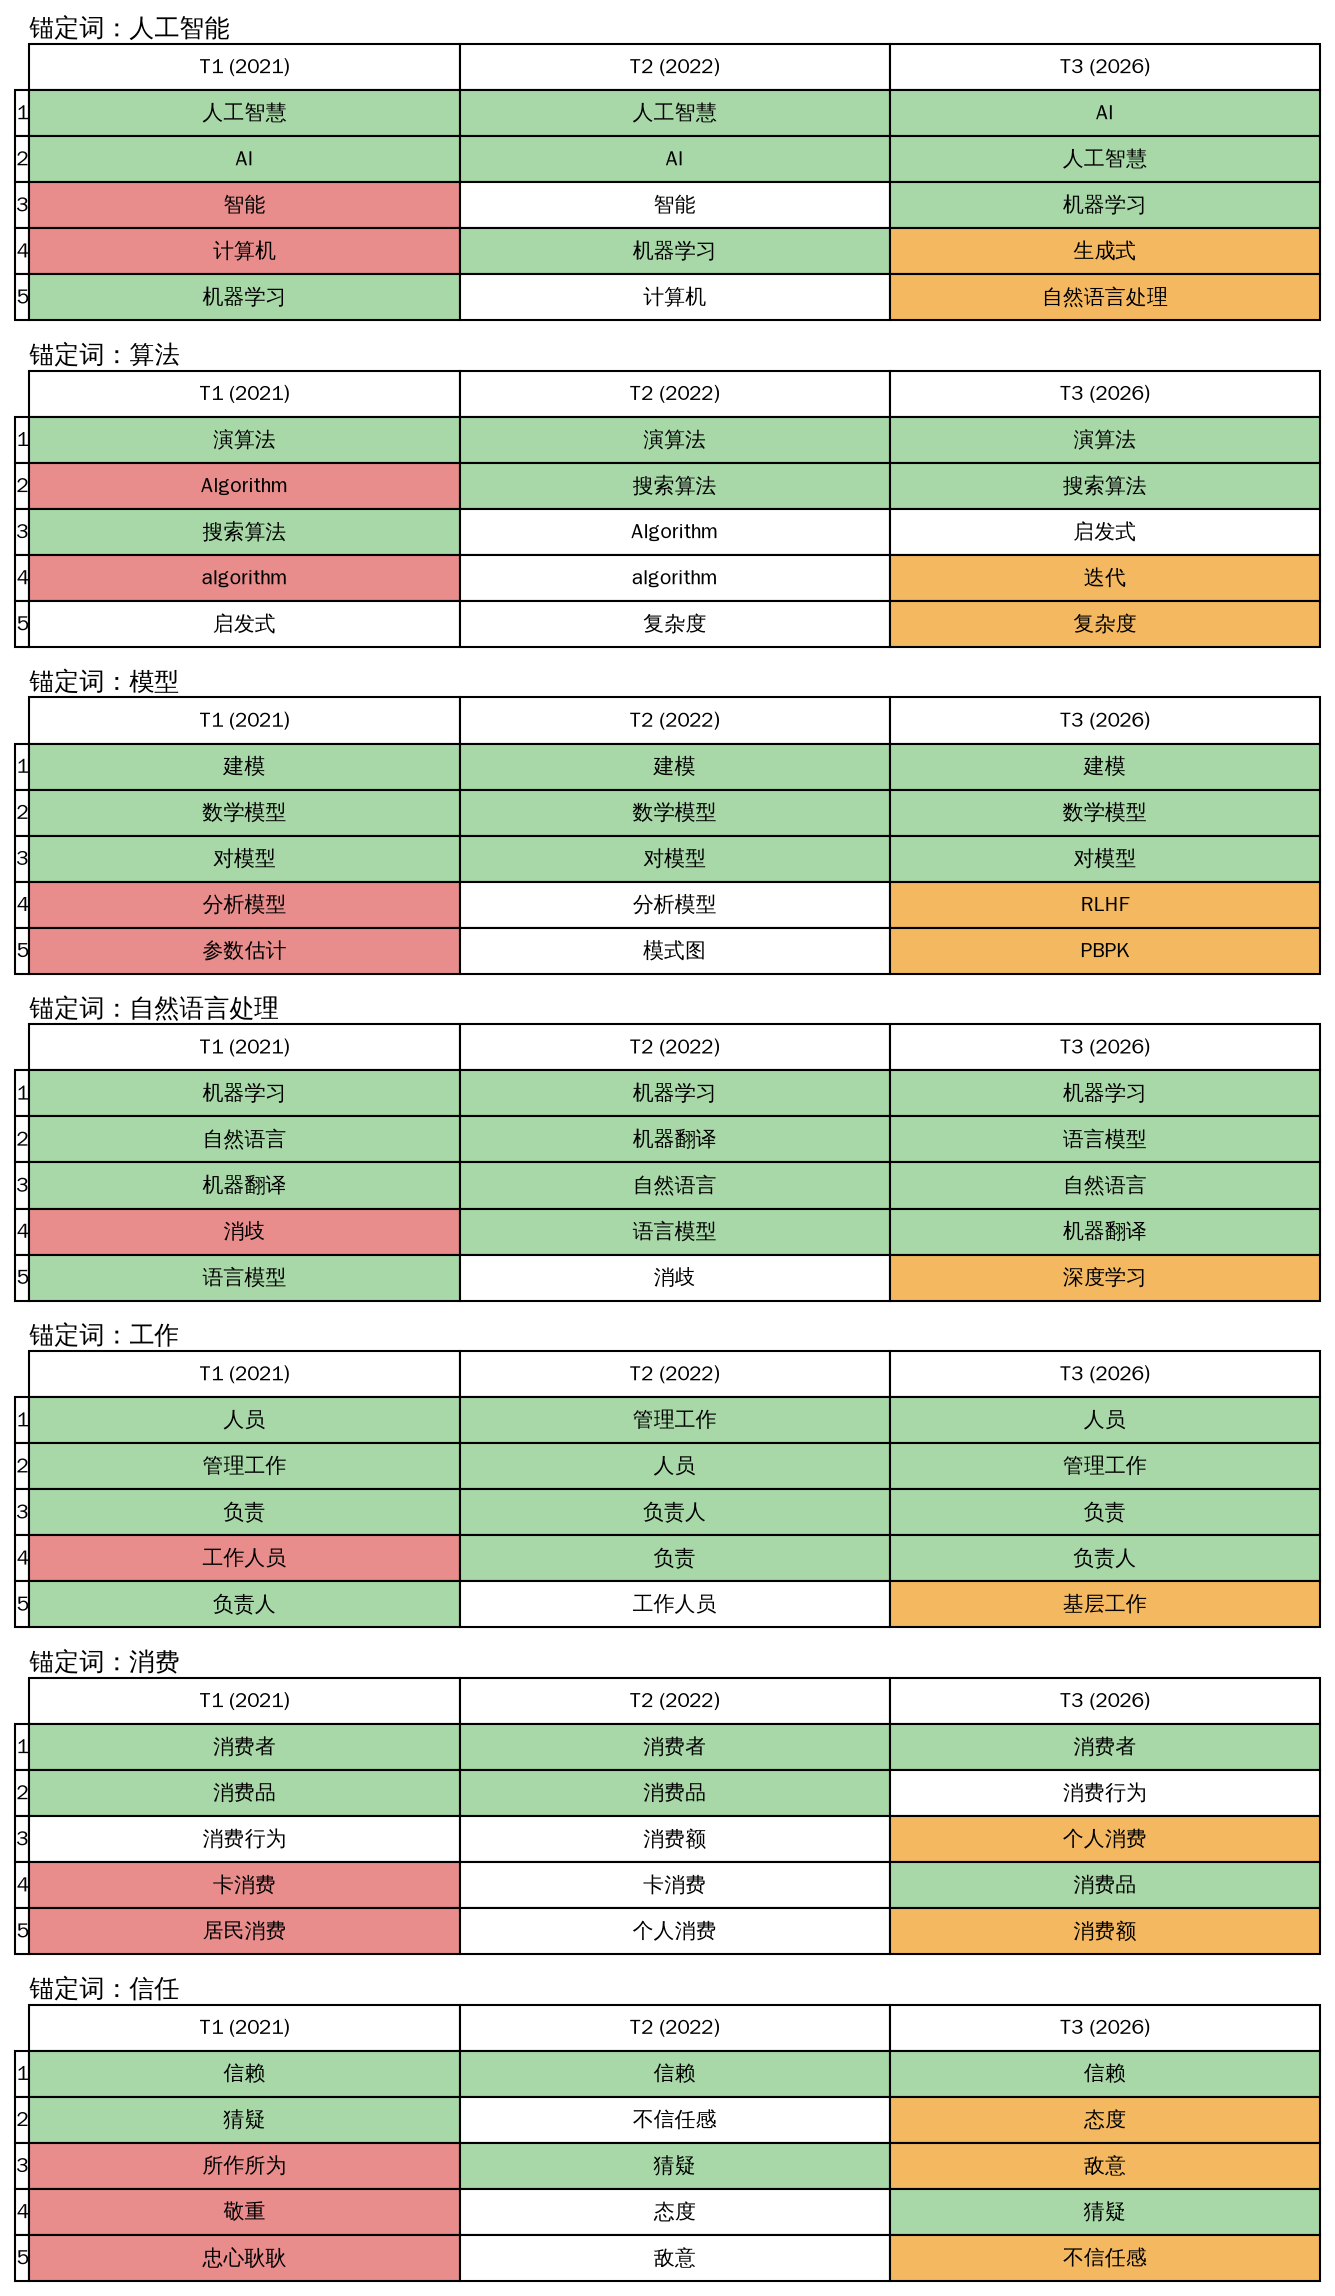
\includegraphics[width=0.96\textwidth]{outputs/figures/fig3_top5_neighbors.png}
\caption{7 个锚定词 Top-5 近邻三时段并排对比（颜色：绿=持续，橙=新出现，红=消失）}
\end{figure}

\subsubsection*{T1 与 T3 Top-5 重合个数（仅作描述性辅助）}

\begin{table}[H]
\centering
\renewcommand{\arraystretch}{1.25}
\begin{tabular}{|l|c|l|}
\hline
\textbf{锚定词} & \textbf{T1$\cap$T3} & \textbf{角色} \\
\hline
人工智能 & 3/5 & 技术（核心） \\
\hline 算法 & 3/5 & 技术（核心） \\
\hline 模型 & 3/5 & 技术（核心） \\
\hline 自然语言处理 & 4/5 & 技术（核心，低频） \\
\hline 工作 & 4/5 & 社会（对照） \\
\hline 消费 & 3/5 & 社会（对照） \\
\hline 信任 & 2/5 & 社会（对照） \\
\hline
\end{tabular}
\end{table}

\textbf{重合个数仅作描述性辅助，不做推断统计。}技术词并非一律比社会词变化更大——“自然语言处理”因低频而近邻偏稳，“信任”因情感词跳变而偏动。定性解读以成员变化方向为准。

\subsubsection{TF-IDF 余弦相似文本检索（对应任务 5）}

在 T3（2026）全量语料上拟合 TF-IDF，对 3 条自拟查询文本返回 Top-5 相似文本（\texttt{code/06\_tfidf\_similarity.py}）。检索结果见下表节选（完整结果 \texttt{outputs/tables/similar\_t3.csv}）：

\begin{table}[H]
\centering
\caption{TF-IDF 余弦相似文本检索 Top-1 / Top-2 结果（查询文本见正文）}
\renewcommand{\arraystretch}{1.25}
\footnotesize
\begin{tabularx}{\textwidth}{|c|X|l|c|}
\hline
\textbf{查询} & \textbf{查询文本（节选）} & \textbf{Top-1 标题} & \textbf{余弦} \\
\hline
Q1 & 大语言模型是深度学习背景下发展起来的一类神经网络语言模型… & 深度学习 & 0.4117 \\
\hline
Q2 & 推荐算法通过用户行为数据预测偏好，被广泛用于短视频、电商… & 上海国际短视频中心 & 0.4038 \\
\hline
Q3 & 灵活就业与远程办公改变了传统的工作模式，劳动者面临收入不稳定… & 中华人民共和国社会保障卡 & 0.3684 \\
\hline
\end{tabularx}
\end{table}

\textbf{排序理由}：Q1 与 T3“深度学习”条目在“深度学习 / 神经网络 / 表征学习 / 算法”等关键 token 上完全重合；Q2 检索回的“上海国际短视频中心”恰好在查询的“短视频 / 电商 / 直播”维度上高频共现——之所以能胜过“算法”条目本身，是因为 TF-IDF 仅以词频维度排序，而 Q2 明显是产业语境而非计算机科学语境；Q3 的高权重词“社会保障 / 就业”与“中华人民共和国社会保障卡”高度重合。

\textbf{方法局限}：TF-IDF 余弦相似度只捕捉\textbf{词汇重叠}，无法处理同义词，也无法反映“同一个词在不同时段语义位置不同”。例如 Q1 查询包含“大语言模型”，但 T3 词表中与之最相似的并非“大语言模型”条目本身（Top-1 是“深度学习”），而只是因为“深度学习”条目里“神经网络 / 算法 / 表征学习”这些 token 重叠度高——这恰恰说明 TF-IDF 无法触及\textbf{语义层}。这一局限正是 6.2.2 节 Word2Vec 近邻分析的必要性所在，两者是\textbf{互补关系}而非替代关系。

\subsubsection{时段分类建模（对应任务 6）}

\textbf{防泄露三条}：①\texttt{period} 标签只用于评估，绝不拼进参与训练的文本；②TF-IDF 只在训练集上 \texttt{fit}，再 \texttt{transform} 测试集；③按文档（行）分层抽样划分，保证同一篇文档不跨训练/测试集，且三个时段的训练/测试比例一致（每段 80,000 篇，8:2 划分）。

\begin{lstlisting}
# load_balanced 三时段各采样 80000，共 240000 篇
texts, labels, titles = load_balanced(max_per_period=80000)
X_train, X_test, y_train, y_test, *_ = train_test_split(
    texts, labels, titles,
    test_size=0.2, random_state=42, stratify=labels)   # 分层划分
vec = TfidfVectorizer(tokenizer=_space_tokenizer, token_pattern=None,
                      max_df=0.85, min_df=5, max_features=50000,
                      ngram_range=(1, 1), lowercase=False)
X_train_vec = vec.fit_transform(X_train_tok)    # 仅训练集 fit
X_test_vec  = vec.transform(X_test_tok)         # 测试集只 transform
\end{lstlisting}

多数类基线 \texttt{accuracy} = \texttt{max(class\_counts)/total} = 80,000/240,000 $\approx$ 0.3333（采样到三段均衡）。

\subsection{结果展示}

\subsubsection*{（1）分类器准确率}

\begin{table}[H]
\centering
\caption{三分类准确率（\texttt{outputs/tables/classification\_summary.csv}）}
\renewcommand{\arraystretch}{1.25}
\begin{tabular}{|l|c|c|c|}
\hline
\textbf{模型} & \textbf{Accuracy} & \textbf{基线（多数类）} & \textbf{提升} \\
\hline
MultinomialNB & 0.3678 & 0.3333 & +0.0344 \\
\hline LinearSVC  & 0.3625 & 0.3333 & +0.0292 \\
\hline
\end{tabular}
\end{table}

\subsubsection*{（2）LinearSVC 完整分类报告（来源：\texttt{logs/07\_classify.log}）}

\begin{table}[H]
\centering
\renewcommand{\arraystretch}{1.25}
\begin{tabular}{|l|c|c|c|c|}
\hline
\textbf{类别} & \textbf{Precision} & \textbf{Recall} & \textbf{F1} & \textbf{Support} \\
\hline
2021 & 0.3447 & 0.3649 & 0.3545 & 16,000 \\
\hline 2022 & 0.3204 & 0.3134 & 0.3168 & 16,000 \\
\hline 2026 & 0.4249 & 0.4093 & 0.4170 & 16,000 \\
\hline
\textbf{macro avg} & 0.3633 & 0.3625 & 0.3628 & 48,000 \\
\hline
\end{tabular}
\end{table}

\subsubsection*{（3）混淆矩阵（LinearSVC，行=真实，列=预测；\texttt{outputs/tables/confusion\_matrix.csv}）}

\begin{table}[H]
\centering
\renewcommand{\arraystretch}{1.3}
\begin{tabular}{|c|c|c|c|}
\hline
\textbf{真实\,$\backslash$\,预测} & \textbf{2021} & \textbf{2022} & \textbf{2026} \\
\hline
\textbf{2021} & 5,839 & 5,952 & 4,209 \\
\hline \textbf{2022} & 6,334 & 5,014 & 4,652 \\
\hline \textbf{2026} & 4,768 & 4,684 & \textbf{6,548} \\
\hline
\end{tabular}
\end{table}

\textbf{关键观察}：两个分类器的 accuracy 仅略高于多数类基线（+3\%），说明三时段全文用词模式差异有限，不足以支撑高精度判别。\textbf{混淆最严重方向是 2022$\rightarrow$2021（6,334 例）}，符合预期——相邻时段最难区分。T3 召回率最高（6,548/16,000 = 40.9\%），反映 T3 新增条目（大模型、生成式 AI 等）带来更多可区分特征。

\subsubsection*{（4）错分样本分析（\texttt{outputs/tables/misclassification\_analysis.csv}）}

\textbf{样本 1：真实 2021 $\rightarrow$ 预测 2026，标题“撞击事件”}
Top TF-IDF 词：撞击(0.72) / 地球(0.305) / 事件(0.24) / 小行星(0.224) / 陨石(0.203) / 彗星(0.187) / 灭绝(0.131) / 陨石坑(0.13)。

\textit{错分原因}：该条目是自然科学主题，使用“撞击 / 小行星 / 陨石”等跨时段稳定的术语，没有任何时段标志性词（既没有 2021 年特有的政治/历史事件词，也没有 2026 年特有的“大模型 / 生成式”词），TF-IDF 高权重词缺乏时段区分性。这暴露了 TF-IDF “只看词面、不看语境”的局限。

\textbf{样本 2：真实 2021 $\rightarrow$ 预测 2022，标题“冠一”}
Top TF-IDF 词：通用(0.499) / 飞机(0.45) / 研制(0.235) / 技术(0.15) / 航空(0.15) / 民营(0.145) / 螺旋桨(0.145) / 有限公司(0.132)。

\textit{错分原因}：这是企业条目，使用“通用 / 飞机 / 研制 / 航空”这类跨 2021—2022 高度相似的产业词汇。2021 与 2022 仅相隔 11 个月，企业条目几乎不变，模型无法在词面上区分。

\textbf{样本 3（来自 \texttt{logs/07\_classify.log}）：真实 2022 $\rightarrow$ 预测 2021，标题“武汉地铁集团”} Top TF-IDF 词：武汉市(0.514) / 武汉(0.418) / 地铁(0.346) / 轨道交通(0.329) / 号线(0.200) / 万人次(0.188) / 线路(0.181) / 运营(0.177)。仍属于跨时段稳定的城市基建主题，再次印证“缺乏时段区分性词”是相邻时段混淆的主因。

\textbf{改进方向}：① 增加时间敏感词特征（如 T3 新进的“大模型 / RLHF / 生成式 / ChatGPT”），可通过自定义二元词典 + \texttt{ngram\_range=(1,2)} 试点；② 引入 LDA 主题分布作为附加特征；③ 把分类目标从“单文本时段”改为“时段分布”，因为相邻时段条目确实在词面层难以区分；④ 用 fastText 或 BERT-style 短文本编码器替代 TF-IDF（拓展部分）。

% ====================== 七、结论与展望 ======================
\section{结论与展望}

\subsection{主要发现}

\begin{enumerate}[leftmargin=2em,itemsep=2pt]
  \item \textbf{时段分类层面}：在本文语料与时段划分下，MultinomialNB / LinearSVC 的准确率分别为 0.3678 / 0.3625，仅略高于多数类基线（+0.034 / +0.029）。三时段全文用词模式差异有限，混淆最严重方向是 2022$\rightarrow$2021（6,334 例），相邻时段条目在词面上难以区分；T3（2026）召回率最高（40.9\%），源于 T3 新增条目带来的可区分特征。
  \item \textbf{Word2Vec 近邻层面}：技术锚定词“人工智能”“模型”的 Top-5 中均出现内容相关的新进入词（“生成式”“自然语言处理”“RLHF”），社会对照词“工作”的 Top-5 高度稳定（4/5 持续近邻）。这一对比性结果\textbf{排除了“全局训练随机性导致所有词都变”的替代解释}，支持技术词近邻变化具有内容相关性的判断。但这是\textbf{探索性观察而非总体推断}：受维基百科语料的来源代表性、年度切片粒度（缺少 2023）、T2$\rightarrow$T3 跨度长达 4 年，以及 Word2Vec 训练随机性限制，不能归因于 ChatGPT 本身。
  \item \textbf{方法互补性}：TF-IDF + 余弦相似检索在 Q1 查询（“大语言模型是深度学习背景下发展起来…”）中返回 Top-1 = “深度学习”条目（余弦 0.4117），而非“大语言模型”条目本身，说明 TF-IDF 无法触及语义层；Word2Vec 则能在“模型”的近邻中捕捉到“RLHF”这一隐性共现关系。两者检验的是不同层面的语义变化，互为补充。
\end{enumerate}

\subsection{项目不足}

\begin{enumerate}[leftmargin=2em,itemsep=2pt]
  \item \textbf{语料代表性}：维基百科不等于中文互联网，编辑群体与内容规范与社交媒体、新闻评论存在系统性差异；观察到的近邻变化是\textbf{百科话语}层面，不能直接推广到日常语言。
  \item \textbf{时段缺失}：原计划四时段，实际因 Wikimedia 技术维护导致 2023 年快照不可获取，仅收集 T1（2021）、T2（2022）、T3（2026）三段，\textbf{缺少后 ChatGPT 关键年（2023）}，无法区分渐变与突变；T2$\rightarrow$T3 跨度长达 4 年，时间粒度粗。
  \item \textbf{方法局限}：不做向量对齐意味着只能比较近邻成员、不能比较相似度数值；Word2Vec 静态词向量无法处理一词多义；近邻列表对词频与训练随机性敏感；\texttt{workers>1} 引入的非确定性通过双 seed 复核缓解，但未做推荐方案的 5 seed 全量复核。
  \item \textbf{混杂因素}：T3 文档数比 T1 多 42\%（658,288 vs 463,376），新增条目可能本身就改变了近邻分布；近邻变化可能部分来自语料主题构成的变化，而非词义本身的变迁。
  \item \textbf{分类任务设计}：从大规模语料均衡采样 80,000 篇避免了规模偏差，但相邻时段的百科条目本身在词面上区分度极低，分类任务在该语料上接近天花板。
\end{enumerate}

\subsection{改进方向}

\begin{enumerate}[leftmargin=2em,itemsep=2pt]
  \item \textbf{补全 2023 时段}：通过 WikiTeam / WikiDump 等第三方镜像进一步搜索 2023 年快照，或在 Internet Archive 上做更细粒度（按月）的检索。
  \item \textbf{引入向量对齐}：参考 Hamilton et al. (2016) 的 Orthogonal Procrustes 对齐，在跨空间相似度可比后做更精细的偏移排序，但仍需注意“可比 $\neq$ 因果”。
  \item \textbf{替换为上下文词向量}：用 BERT-wwm / MacBERT 在各时段语料上做微调，对锚定词在具体上下文中的表示做历时比较，缓解一词多义问题。
  \item \textbf{多语料对照}：加入微博 / 知乎等社交媒体语料（合规渠道），检验“百科话语”与“日常话语”的变迁模式是否一致。
  \item \textbf{分类任务升级}：把三分类改为“pre-ChatGPT vs post-ChatGPT”二分类，或加入半监督方法利用未标注条目；引入 fastText 子词嵌入做对照。
\end{enumerate}

% ====================== 八、项目总结与心得体会 ======================
\section{项目总结与心得体会}

整个项目从选题到完成，让我对“数据采集与处理”这门课各周的内容有了体系化的实战体验。第 1—4 周的合规采集与 Pandas 清洗、第 5 周的 CSS 选择器与 XPath 对比、第 6—7 周的 jieba 分词与停用词、第 8—10 周的 TF-IDF 与分类建模、第 11 周的 Word2Vec——这些原本分散的知识点在“历时语义变迁”这一条主线上被串起来了，我也第一次切实体会到“特征工程的每一步都会被下游模型放大”这句话：jieba 精确模式与全模式的差异，在分类阶段看不太出来，到了 Word2Vec 近邻结构里就被显著放大，所以选精确模式不是“标准答案”，而是被分析对象倒逼出来的选择。

合规获取与学术规范是我在这个项目里反思最多的一块。最初我也考虑过爬维基百科在线版按月归档，但读到一个反直觉的细节——Wikimedia 官方明确鼓励通过 dump 而非在线抓取获取批量内容，在线抓取反而更可能违反其服务条款——就改成了 dump + WikiExtractor 的离线方案。我意识到，“合规”并不总是“抓得越少越好”或“抓得越多越能干”，而是要在数据规模、来源合法性、可复现性三者之间找平衡：dump 是固定快照，保证可复现；CC BY-SA 4.0 是合规协议，保证可公开；离线文件不触反爬，保证不越线。这种“在约束下做诚实研究”的判断力，本身就是课程希望训练的核心能力。

学术规范的另一面是“不把结果包装成结论”。Word2Vec 没做向量对齐，跨空间相似度数值不可比，我就只比较 Top-5 近邻成员；Top-5 重合个数会被误读为“偏移量”，我就在表下明确写“描述性辅助，不做推断统计”；观察到“RLHF”进入“模型”近邻很诱人想下“ChatGPT 改变了技术语义”的结论，但 T3 文档数比 T1 多 42\%、缺少 2023 时段、训练有随机性——这些混杂因素必须如实写进 7.2，措辞只能落在“探索性观察”。这种“自我设限”看起来在削弱结论，但实际上是在保护结论不被反驳。

最后，我也看到了项目本身的局限：5 seed 稳健近邻只做了 2 seed、2023 时段补不回来、维基百科编辑群体不能代表中文互联网全貌。这些不足不会因为不提就消失，写进 7.2 反而让结论更有说服力。下一次做类似研究，我会优先补全时段、引入上下文词向量，并把“百科话语”与日常语料做并行对照。

% ====================== 九、附录 ======================
\section{附录：完整代码清单}

\begin{table}[H]
\centering
\renewcommand{\arraystretch}{1.25}
\begin{tabularx}{\textwidth}{|l|X|}
\hline
\textbf{文件} & \textbf{功能} \\
\hline
\texttt{code/utils.py} & 固定随机种子 \texttt{SEED=42}，设置 \texttt{random.seed}、\texttt{np.random.seed} 与 \texttt{PYTHONHASHSEED} 环境变量 \\
\hline
\texttt{code/01\_extract.py} & 调用 WikiExtractor 3.1.0 从 \texttt{*.xml.bz2} 提取纯文本，自动检测 export-0.10 / 0.11 命名空间，过滤 \texttt{ns=0} 之外页面与正文长度 $<200$ 的条目 \\
\hline
\texttt{code/02\_postprocess.py} & 中文后处理：全角$\rightarrow$半角、繁$\rightarrow$简（OpenCC \texttt{t2s}）、空白合并、长度 $<200$ 过滤、MD5 去重；输出 \texttt{data/processed/zhwiki\_\{period\}.jsonl} \\
\hline
\texttt{code/03\_tokenize.py} & jieba 精确模式 + 20 个领域自定义词典分词；哈工大+百度停用词表合并过滤；每段独立拟合 TF-IDF 并输出 Top-20 关键词与锚定词词频核查 \\
\hline
\texttt{code/04\_train\_word2vec.py} & 分时段独立训练 Word2Vec（200 维 / window=8 / min\_count=10 / sg=1 / 10 epochs），支持双 seed 复核；输出 \texttt{w2v\_\{period\}\_seed\{S\}.kv} \\
\hline
\texttt{code/05\_top5\_neighbors.py} & 聚合多 seed 模型提取“稳健 Top-5 近邻”，生成 \texttt{top5\_neighbors\_by\_period.csv}（长表）与 \texttt{top5\_comparison.csv/.md}（并排对比，含标注） \\
\hline
\texttt{code/06\_tfidf\_similarity.py} & 在 T3 语料上用 TF-IDF 余弦相似检索 3 条自拟查询的 Top-5 文本；输出 \texttt{similar\_t3.csv} \\
\hline
\texttt{code/07\_period\_classify.py} & 均衡采样 80,000/段共 240,000 篇，8:2 分层划分，TF-IDF 仅在训练集 fit，训练 MultinomialNB 与 LinearSVC 三分类器，输出准确率、分类报告、混淆矩阵与错分样本（含 Top TF-IDF 词） \\
\hline
\texttt{code/08\_visualize.py} & 生成 3 张图：\texttt{fig1\_doc\_counts.png}（文档数柱状图）、\texttt{fig2\_text\_length.png}（正文长度小提琴图）、\texttt{fig3\_top5\_neighbors.png}（锚定词 Top-5 变化着色表） \\
\hline
\texttt{requirements.txt} & 锁定依赖：\texttt{wikiextractor==3.1.0}、\texttt{opencc-python-reimplemented==0.1.7}、\texttt{jieba==0.42.1}、\texttt{gensim==4.4.0}、\texttt{scikit-learn==1.9.1}、\texttt{pandas==3.1.1}、\texttt{numpy==2.5.5}、\texttt{matplotlib==3.11.2}、\texttt{seaborn==0.13.2} 等 \\
\hline
\texttt{README.md} & 运行顺序、各时段 dump 日期与下载链接、环境与依赖版本、随机种子说明、报告中每个数字对应的输出文件路径 \\
\hline
\end{tabularx}
\end{table}

\subsubsection*{运行顺序}

\begin{lstlisting}[language=bash, basicstyle=\ttfamily\footnotesize]
python code/01_extract.py 2021       # 三时段分别执行
python code/02_postprocess.py 2021   # 三时段分别执行
python code/03_tokenize.py 2021      # 三时段分别执行
python code/04_train_word2vec.py all --seeds 42 43
python code/05_top5_neighbors.py
python code/06_tfidf_similarity.py
python code/07_period_classify.py --max-per-period 80000
python code/08_visualize.py
\end{lstlisting}

\subsubsection*{报告数字与代码输出对应关系}

\begin{itemize}[leftmargin=2em,itemsep=0pt]
  \item 3.3 各时段文档数 463,376 / 508,512 / 658,288 $\leftrightarrow$ \texttt{logs/03\_tokenize.log} 输入统计
  \item 4.4 分词前后词表 2,982,493 / 2,960,669 $\leftrightarrow$ \texttt{logs/03\_tokenize.log}
  \item 5.3 Top-20 TF-IDF 关键词 $\leftrightarrow$ \texttt{outputs/tables/tfidf\_top20\_2021.csv} / \texttt{\_2022.csv} / \texttt{\_2026.csv}
  \item 5.3 / 6.2 锚定词词频 $\leftrightarrow$ \texttt{logs/04\_word2vec.log} + \texttt{logs/04\_word2vec\_t3.log}
  \item 6.2 Top-5 近邻 $\leftrightarrow$ \texttt{outputs/tables/top5\_neighbors\_by\_period.csv} + \texttt{top5\_comparison.csv}
  \item 6.2 相似检索 $\leftrightarrow$ \texttt{outputs/tables/similar\_t3.csv}
  \item 6.3 分类准确率 / 混淆矩阵 / 错分样本 $\leftrightarrow$ \texttt{outputs/tables/classification\_summary.csv} + \texttt{confusion\_matrix.csv} + \texttt{misclassification\_analysis.csv} + \texttt{logs/07\_classify.log}
\end{itemize}

\end{document}
